\documentclass[12pt]{article}

\usepackage{fullpage}
\usepackage{graphicx}
\usepackage{fancybox}
\usepackage{hyperref}
 
\newcommand{\DFSa}{\textsf{\sc DFS}}
\newcommand{\EXPLORE}{\textsf{\sc Explore}}
\newcommand{\UNION}{\textsf{\sc Union}}
\newcommand{\FIND}{\textsf{\sc Find}}

\newcommand{\DFS}{\mathord{\it DFS}}
\newcommand{\PRE}{\mathord{\it pre}}
\newcommand{\POST}{\mathord{\it post}}
\newcommand{\VISITED}{\mathord{\it visited}}
\newcommand{\TRUE}{\mathord{\it true}}
\newcommand{\FALSE}{\mathord{\it false}}
\newcommand{\CLOCK}{\mathord{\it clock}}
\newcommand{\LAS}{\mathord{\it LAS}}

\newcounter{ques}
\newenvironment{question}{\stepcounter{ques}{\noindent\bf Question \arabic{ques}:}}{\vspace{5mm}}
\newenvironment{solution}{{\noindent\bf Solution:}}{\vspace{5mm}}

\begin{document} 

\begin{center} \Large\bf
COMP 3804 --- Assignment 3 
\end{center} 

\noindent {\bf Due:} Thursday March 23, 23:59.

\vspace{0.5em}

\noindent {\bf Assignment Policy:}
\begin{itemize}
\item Your assignment must be submitted as one single PDF file through
      Brightspace.

\begin{center}
\hfill\shadowbox{
  \begin{minipage}{.90\linewidth}
    {\textsf{Use the following format to name your file:
        \[ {\tt LastName\_StudentId\_a3.pdf}
        \]
      }}
  \end{minipage}
}
\end{center}
\item {\bf Late assignments will not be accepted. I will not reply to
      emails of the type ``my internet connection broke down at
      23:57'' or ``my scanner stopped working at 23:58'', or
      ``my dog ate my laptop charger''.}
\item You are encouraged to collaborate on assignments, but at the level
      of discussion only. When writing your solutions, you must do so
      in your own words.
\item Past experience has shown conclusively that those who do not put
      adequate effort into the assignments do not learn the material and
      have a probability near 1 of doing poorly on the exams.
\item When writing your solutions, you must follow the guidelines below.
      \begin{itemize}
      \item You must justify your answers.
      \item The answers should be concise, clear and neat.
      \item When presenting proofs, every step should be justified.
      \end{itemize}
\end{itemize}

\newpage 

\begin{question}
Write your name and student number.
\end{question}

\begin{solution}

      Ryan Lo (101117765)

\end{solution}

\begin{question}  
Consider the following directed graph: 
 
\begin{center}
     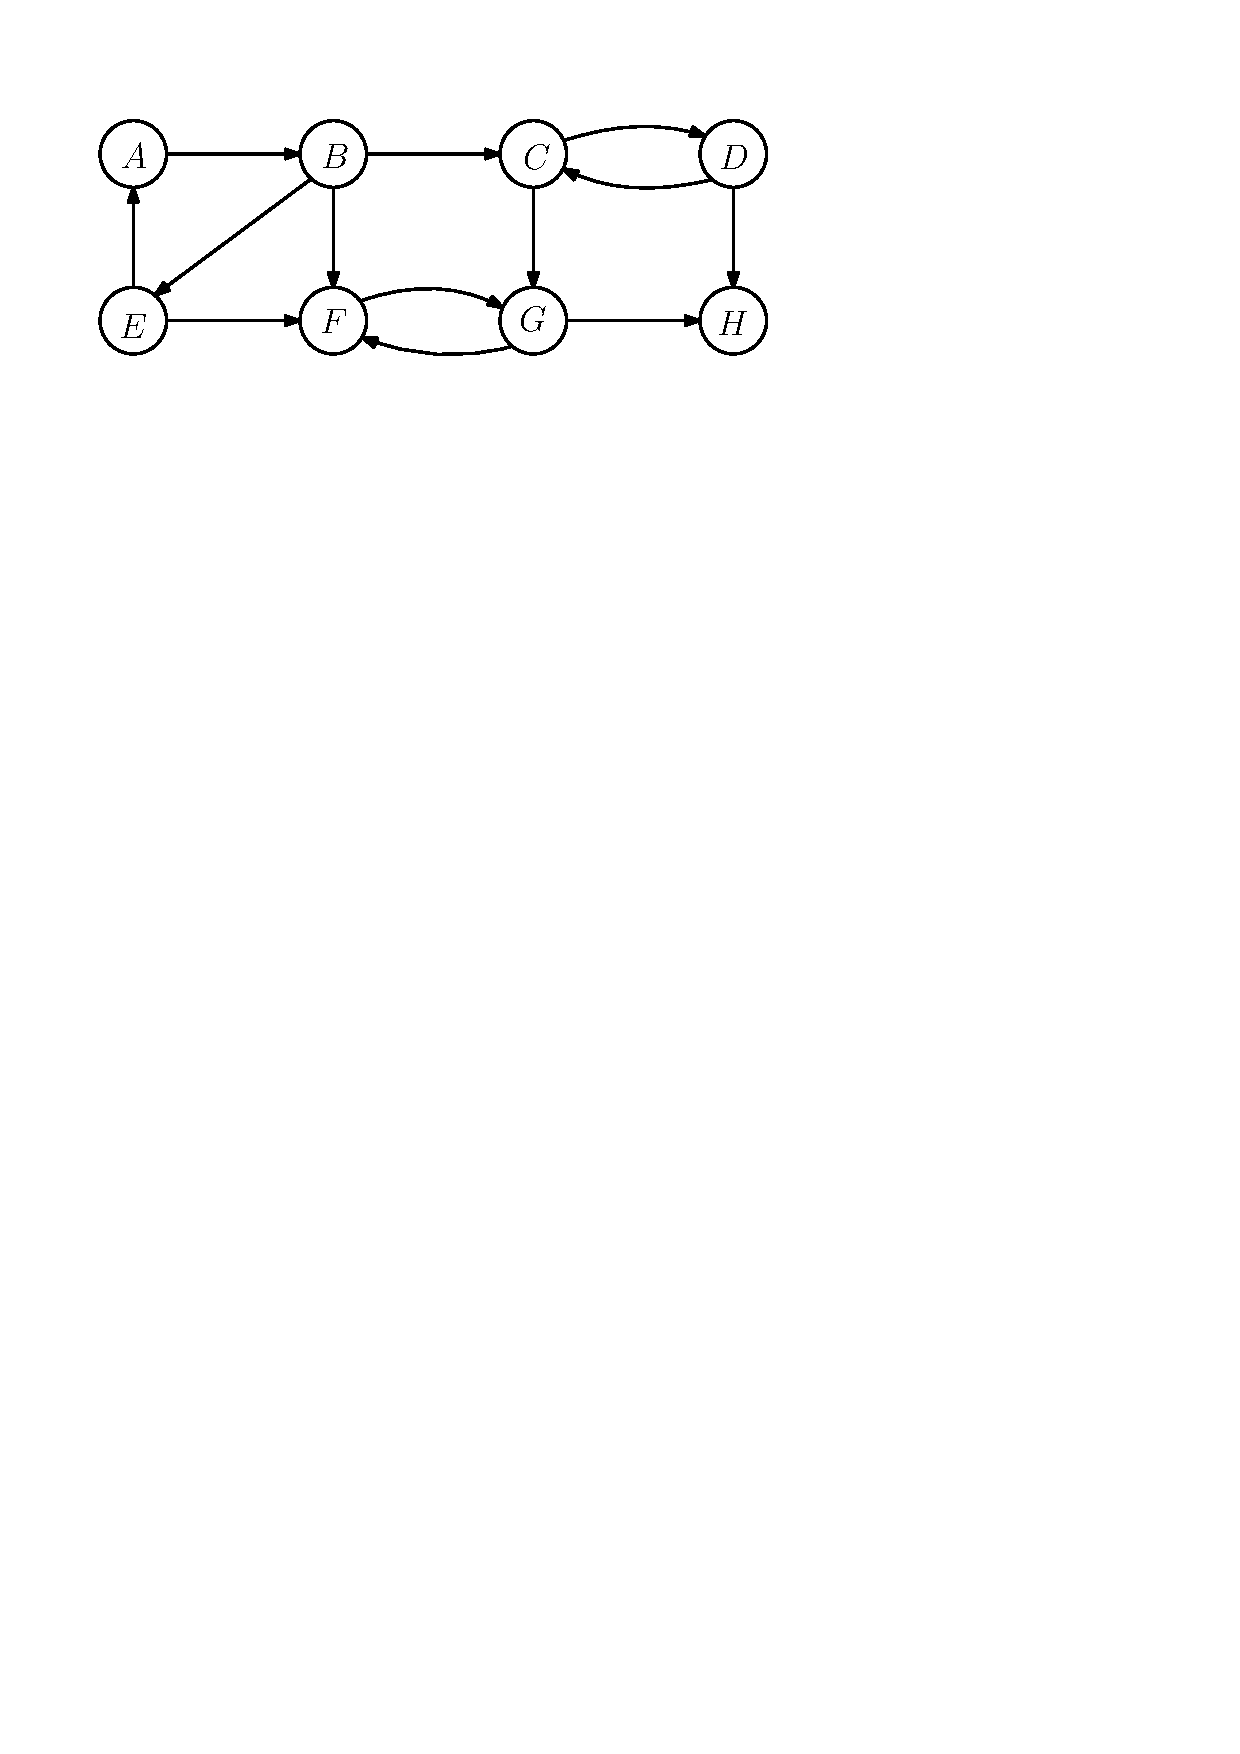
\includegraphics[scale=0.5]{graphA3}
\end{center}

\noindent
{\bf (\arabic{ques}.1)} 
Draw the $\DFS$-forest obtained by running algorithm $\DFSa$. 
Classify each edge as a tree edge, forward edge, back edge, or cross 
edge. In the $\DFS$-forest, give the $\PRE$- and $\POST$-number of each 
vertex. Whenever there is a choice of vertices, pick the one that is 
alphabetically first.     

\vspace{0.5em} 

\begin{solution}
      
      \bf {2.1:}

      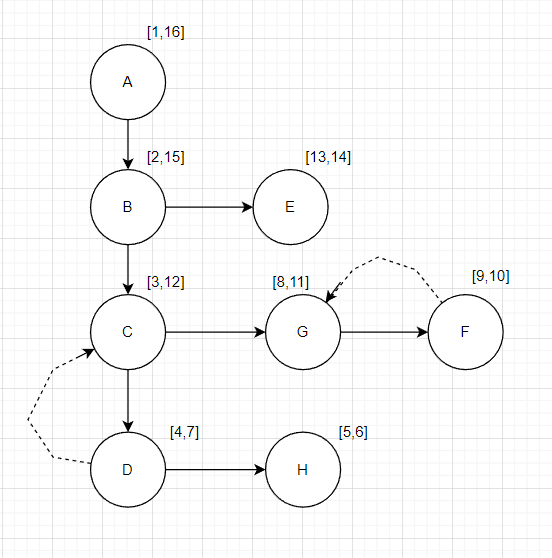
\includegraphics[scale=1]{2.1}

      Tree Edge: {(A,B), (B,C), (C,D), (D,H), (C,G), (G,F), (B,E)}

      Forward Edges: None

      Back Edges: {(D,C), (F,G)}

      Cross Edges: None

      \vspace{0.5em} 

      \bf 2.2:

      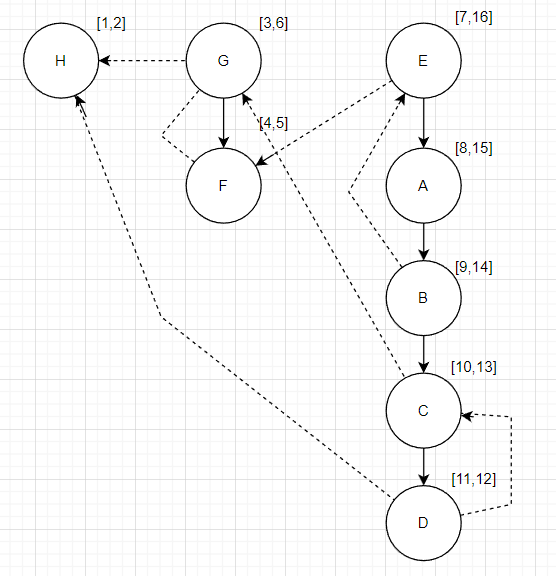
\includegraphics[scale=1]{2.2}

      Tree Edge: {(G,F), (E,A), (A,B), (B,C), (C,D)}

      Forward Edges: None

      Back Edges: {(D,C), (F,G), (B,E)}

      Cross Edges: {(G,H), (D,H), (E,F), (C,G)}

      \vspace{0.5em} 
\end{solution}

\noindent
{\bf (\arabic{ques}.2)} 
Draw the $\DFS$-forest obtained by running algorithm $\DFSa$. 
Classify each edge as a tree edge, forward edge, back edge, or cross 
edge. In the $\DFS$-forest, give the $\PRE$- and $\POST$-number of each 
vertex. Whenever there is a choice of vertices, pick the one that is 
alphabetically last.     
\end{question} 

\begin{quote}
\begin{tabbing}
{\bf Algorithm} $\DFSa(G)$: \\
{\bf for each} vertex $v$ \\
{\bf do} $\VISITED(v) = \FALSE$ \\
{\bf endfor}; \\
$\CLOCK = 1$; \\
{\bf for each} vertex $v$ \\
{\bf do} \= {\bf if} $\VISITED(v) = \FALSE$ \\
         \> {\bf then} $\EXPLORE(v)$  \\
         \> {\bf endif} \\
{\bf endfor} \\
\end{tabbing}
\end{quote}

\begin{quote}
\begin{tabbing}
{\bf Algorithm} $\EXPLORE(v)$: \\
$\VISITED(v) = \TRUE$; \\
$\PRE(v) = \CLOCK$; \\
$\CLOCK = \CLOCK + 1$; \\
{\bf for each} edge $(v,u)$ \\
{\bf do} \= {\bf if} $\VISITED(u) = \FALSE$ \\
         \> {\bf then} \= $\EXPLORE(u)$ \\
         \> {\bf endif} \\
{\bf endfor}; \\
$\POST(v) = \CLOCK$; \\
$\CLOCK = \CLOCK + 1$ \\
\end{tabbing}
\end{quote}


\begin{question}
Let $G=(V,E)$ be a directed graph. After algorithm $\DFSa(G)$ has 
terminated, each vertex has a $\PRE$- and $\POST$-number. 
Let $u$ and $v$ be two distinct vertices in $V$. Prove the 
following: 

\begin{itemize}
\item If $\PRE(u) < \PRE(v) < \POST(u)$, then there is a directed path 
in $G$ from $u$ to $v$. 
\item Assume that $G$ is directed and acyclic. If $\POST(u) < \PRE(v)$, 
then there is no directed path in $G$ from $u$ to $v$. 
\end{itemize}
\end{question}

\begin{solution}
      
      If pre(u) $<$ pre(v) $<$ post(u), then there is a directed path in $G$ from $u$ to $v$.
      Proof by contradiction:
      Assume there is no directed path from $u$ to $v$. Then there exists no path from $u$ to $v$, or there exists a path from $v$ to $u$. In the first case, $v$ is not reachable from $u$, which contradicts the fact that pre(v) $>$ pre(u). 
      In the second case, $u$ is not reachable from $v$, which implies that post(u) $>$ post(v), which again contradicts the given condition that pre(v) $<$ post(u). 
      Therefore, there must be a directed path from $u$ to $v$.

      Assume that G is directed and acyclic. If post(u) $<$ pre(v), then there is no directed path in G from $u$ to $v$.
      Proof by contradiction:
      Assume that there exists a directed path from $u$ to $v$. 
      Since G is acyclic, this path must be simple, meaning that it does not contain any cycles and repeated vertices. 
      Let w be the last vertex on this path that is visited before v. 
      Then, there is a path from u to w that does not include v, and since w is visited before v, we have pre(w) $<$ pre(v). 
      Also, since w is the last vertex visited before v, we have post(w) $>$ post(v). 
      Therefore, we have pre(u) $<$ pre(w) $<$ post(w) $<$ post(v) $<$ post(u), which contradicts the fact that G is acyclic. 
      Therefore, there is no directed path from $u$ to $v$ in G if post(u) $<$ pre(v).
\end{solution}

\begin{question}
Let $n \geq 2$ be an integer and let $G$ be the $n \times n$ undirected 
grid graph: The vertices of $G$ are the grid points $(i,j)$ for 
$1 \leq i \leq n$ and $1 \leq j \leq n$. Each vertex $(i,j)$ has 
neighbors $(i-1,j)$, $(i+1,j)$, $(i,j-1)$, and $(i,j+1)$ (provided 
their coordinates are in the set $\{1,2,\ldots,n\}$). 

Each vertex of this graph stores a number; we assume that all these 
$n^2$ numbers are distinct. A vertex is called \emph{awesome}, 
if the number stored at this vertex is larger than the numbers stored 
at all of its neighbors. In the example below, $n=4$ and both vertices 
$(1,1)$ and $(3,2)$ are awesome. 

\begin{center}
     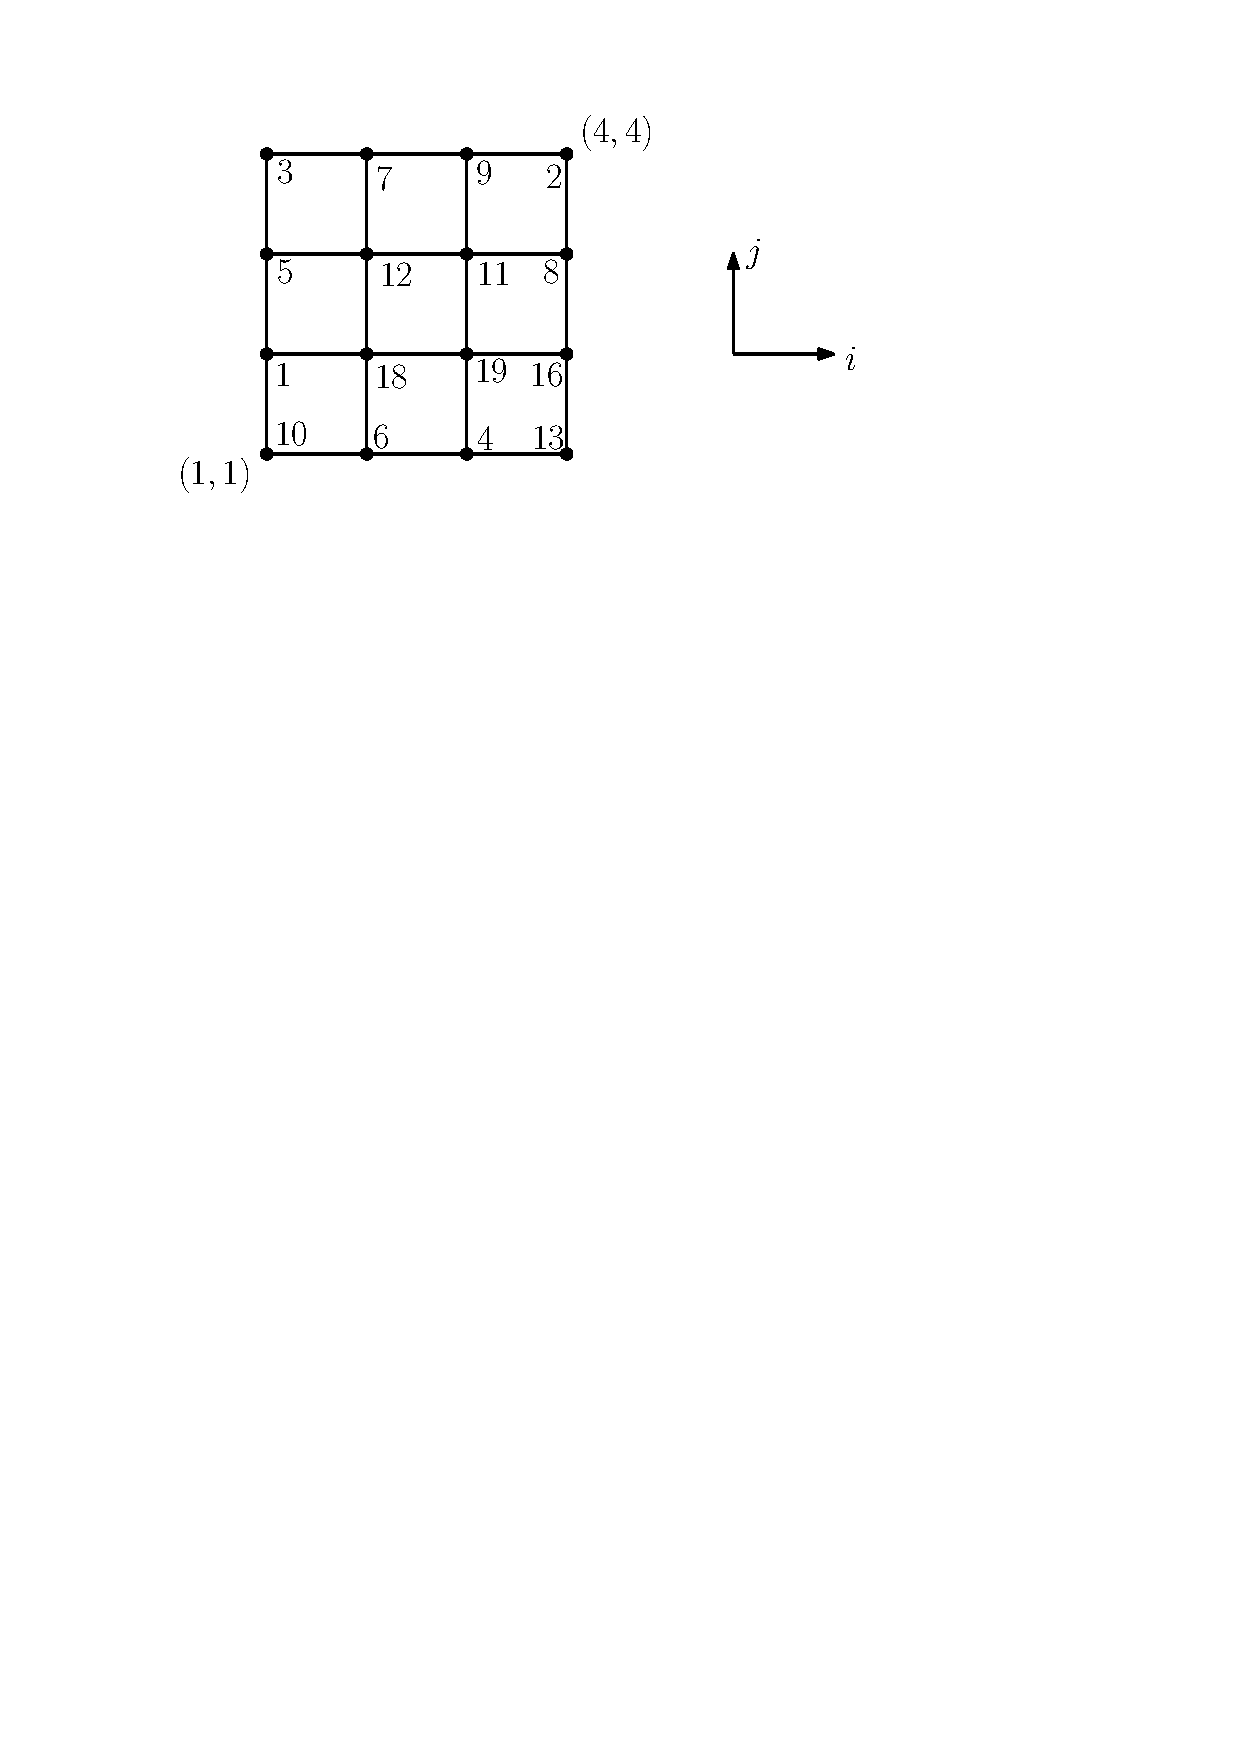
\includegraphics[scale=0.7]{grid}
\end{center}

\begin{itemize} 
\item Prove that there always exists at least one awesome vertex.
\item Give an algorithm that finds an awesome vertex in $O(n)$ time. 
Note that the graph $G$ has $n^2$ vertices and $\Theta(n^2)$ edges. 
\end{itemize} 
\end{question} 

\begin{solution}
      
      Whatever the largest number in the grid graph is must be an awesome vertex because every other neighbor must be less than it making the largest vertex an awesome vertex.
      Another way to look at this is, let $x$ be the vertex with the maximum number among all the vertices of G. 
      If $x$ is awesome, we are done. Otherwise, at least one of $x$'s neighbors must be awesome, because x's neighbors are the only vertices that can potentially be larger than x. 
      We can then repeat the process with the awesome neighbor(s) until we find an awesome vertex. 
      Since each step reduces the number of candidate vertices by at least one, and there are only finitely many vertices in G, this process must eventually terminate with the discovery of an awesome vertex.

      We can find an awesome vertex in O(n) time by starting at vertex (1, n), which is the top-right corner of the grid, and traversing the grid row-by-row from right to left. 
      At each vertex (i, j), we compare its number to the numbers of its right and bottom neighbors. 
      If (i, j) has the largest number among these three vertices, it is awesome and we return it. 
      Otherwise, we find the neighbor with the largest number. If that number is larger than the number at the current vertex, we move to that neighbor. 
      Otherwise, we move down to the neighbor below (i, j). 
      Since there are at most n rows, every step eliminates at least 2 vertices which means the time complexity of this algorithm is O(n).
\end{solution}

\begin{question} 
Let $G=(V,E)$ be a directed acyclic graph that is given to you using 
adjacency lists. We say that $G$ is \emph{nice} if for every two distinct 
vertices $u$ and $v$, there is a directed path from $u$ to $v$, or there 
is a directed path from $v$ to $u$. 

Give an algorithm that decides in $O(|V|+|E|)$ time whether $G$ is nice. 
As always, justify your answer. 

\noindent 
\emph{Hint:} 
Find some examples of directed acyclic graphs with four vertices 
that are nice, and find some examples that are not nice. What 
property of their topological orderings distinguishes them?  
\end{question}

\begin{solution}
      
      To decide whether a directed acyclic graph G is nice, we need to check whether for every two distinct vertices $u$ and $v$, there is a directed path from $u$ to $v$, or there is a directed path from $v$ to $u$. 
      If G has a topological ordering, then it is acyclic, and if G is acyclic, then it has a topological ordering.
      Therefore, we can use the topological ordering of the vertices in G and check whether the ordering satisfies the property of being nice.

      Now, let's consider two distinct vertices $u$ and $v$ in G. 
      If there is a directed path from $u$ to $v$ in G, then in any topological ordering of G, $u$ must come before $v$. 
      Similarly, if there is a directed path from v to u in G, then in any topological ordering of G, $v$ must come before $u$. 
      Thus, G is nice if and only if every pair of distinct vertices $u$ and $v$ in G satisfies either $u$ comes before $v$ or $v$ comes before $u$ in the topological ordering of G.
      To check whether G is nice, we can compute a topological ordering of G and then check whether for every pair of distinct vertices $u$ and $v$, either $u$ comes before $v$ or $v$ comes before $u$ in the ordering. 
      If this property is satisfied, then G is nice; otherwise, G is not nice.
      
      The time complexity of this algorithm is O($|V|$ + $|E|$) to compute the topological ordering of G using depth-first search.
      And the time complexity to check whether or not the topological ordering has a property of being nice is O($|V|$).
      Therefore, the algorithm is correct and runs in O($|V|$ + $|E|$) time.
\end{solution}

\newpage 

\begin{question}
In class, we have seen a data structure for the $\UNION-\FIND$ problem
that stores each set in a linked list, with the header of the list
storing the name and size of the set. Using this data structure, any
operation $\FIND(x)$ takes $O(1)$ time, whereas any operation
$\UNION(A,B,C)$ takes $O(\min(|A|,|B|))$ time.

Consider the same data structure, except that the header of each list
only stores the name of the set (and not the size). Show that, in
this new data structure, any operation $\FIND(x)$ can be performed in
$O(1)$ time, and any operation $\UNION(A,B,C)$ can still be
performed in $O(\min(|A|,|B|))$ time.
\end{question}

\begin{solution}
      
      To show that any operation Find(x) can be performed in O(1) time, we can simply store a pointer to the header node of each linked list in an array of size n, where n is the number of elements in the universe. 
      Given an element x, we can follow the back pointer from the node to the head of the list of its set in O(1) time using the array, and then return the name of the set stored in the header node.

      To show that any operation Union(A, B, C) can still be performed in O(min($|A|$, $|B|$)) time, we can use the same basic idea as the original data structure, but with a slight modification. 
      We can choose one of the sets A and B (say A), and append the nodes of the other set B to the end of A's linked list. Then, we update the header node of B to point to the header node of A.

      To do this efficiently, we need to keep track of which of A and B has the smaller size, say A. 
      Then, we can traverse the linked list of A to find its last node, and append the nodes of B to the end of that list. This takes O($|A|$) time. 
      Finally, we update the header node of B to point to the header node of A, which takes O(1) time. 
      This does not change the name of the set stored in the header node of A.

      Overall, this operation takes O($|A|$) time, which is equal to the minimum of the sizes of A and B, as required. 
      This completes the proof that any operation Union(A, B, C) can be performed in O(min($|A|$, $|B|$)) time in the modified data structure.

      Therefore, we have shown that, even if we only store the name of each set in the header node of its linked list, we can still perform any operation Find(x) in O(1) time and any operation Union(A, B, C) in O(min($|A|$, $|B|$)) time.
\end{solution}

\begin{question} 
A sequence $(b_1,b_2,\ldots,b_k)$ of numbers is called \emph{amazing}, 
if there is an index $i$ with $1 \leq i \leq k$, such that 
$(b_1,b_2,\ldots,b_i)$ is increasing and $(b_i, b_{i+1}, \ldots,b_k)$ 
is decreasing. 

Let $S=(a_1,a_2,\ldots,a_n)$ be a sequence of numbers. Give an algorithm 
that computes, in $O(n^2)$ time, the length $\LAS(S)$ of a longest 
amazing subsequence of $S$. The numbers in the subsequence are not 
necessarily consecutive in $S$. 

For example, if 
\[ S=(10,22,9,33,21,50,41,60,80,1) , 
\]
then $\LAS(S) = 7$, because $(10,22,33,50,60,80,1)$ is a longest amazing 
subsequence. 

As always, argue why your algorithm is correct. You my use any result 
that was presented in class.  
\end{question}

\begin{solution}
      
      We can solve this problem using dynamic programming. 
      Let L1 be an array where L1[i] is the length of the longest amazing subsequence ending at index i of the sequence S.

      To compute L1[i], we iterate over all indices j $<$ i and check if the longest increasing sequence S[j] $<$ S[i]. If so, then we L[i] = L[j] + 1. 
      
      Similarly, we can let L2 be an array where L2[i] is the length of the longest amazing subsequence ending at index i of the sequence S
      and do the same thing as L1 but in reverse order 
      iterate over all indices k $<$ i and check if the longest increasing sequence S[k] $<$ S[i]. If so, then we L[i] = L[k] + 1.

      From the given Example:

      S = (10, 22, 9, 33, 21, 50, 41, 60, 80, 1)

      array1 = [1, 2, 2, 3, 3, 4, 4, 5, 6, 6]

      array2 = [3, 3, 3, 3, 3, 3, 2, 2, 2, 1]

      Once we have computed all the values of L1 and L2, we can take max of array1[i] and array2[i] for all i and subtract by one because of the overlap.

      For the example above it would be L1[8] + L2[8] - 1 = 6 + 2 - 1 = 7
      
      The time complexity of this algorithm is O($n^2$) because we need to iterate over all pairs of indices for each index i.
      
      To prove the correctness of the algorithm, we can use mathematical induction. Let L[i] be the length of the longest amazing subsequence ending at index i, and let LAS(i) be the length of the longest amazing subsequence of S that ends at index i. We want to show that L[i] = LAS(i) for all i.
      
      Base case: L[1] = 1 and LAS(1) = 1 since any subsequence of length 1 is amazing.
      
      Inductive step: Assume that L[j] = LAS(j) for all j $<$ i. We want to show that L[i] = LAS(i).
      
      Case 1: There exists a value j $<$ i such that S[j] $<$ S[i]. In this case, the longest amazing subsequence ending at index i must include S[i], and it can be obtained by extending the longest amazing subsequence ending at index j. Thus, L[i] = L[j] + 1 = LAS(j) + 1 = LAS(i).
      
      Case 2: There exists a value k $>$ i such that S[k] $<$ S[i]. In this case, the longest amazing subsequence ending at index i must include S[i], and it can be obtained by extending the longest amazing subsequence starting at index k. Thus, L[i] = L[k] + 1 = LAS(k) + 1 = LAS(i).
      
      Case 3: There are no values j $<$ i or k $>$ i such that S[j] $<$ S[i] or S[k] $<$ S[i]. In this case, the longest amazing subsequence ending at index i is just S[i] itself, and LAS(i) = 1. Thus, L[i] = 1 = LAS(i).
      
      Since we have shown that L[i] = LAS(i) for all i, the algorithm is correct.
\end{solution}
\newpage
\begin{question} 
After having taken many flights with ZoltanJet, Alma is ready to redeem 
her frequent flyer points: Alma can choose from a wide selection of beers! 
Each beer costs a certain number of points. Of course, being a 
beer connoiseur, each beer has a value to Alma. For example, Heineken has 
a low value, whereas Minerva Stout has a high value. Which beers does 
Alma choose? 

There are $n$ types $B_1,B_2,\ldots,B_n$ of beer. For each $i$ with 
$1 \leq i \leq n$, 
\begin{itemize}
\item it costs $p_i$ points to acquire beer $B_i$, 
\item the value of beer $B_i$ is equal to $v_i$. 
\end{itemize} 
Alma has $P$ points to spend. We denote the beers that she chooses 
by the subset $I \subseteq \{1,2,\ldots,n\}$ of their indices. 
(For each $i$, Alma cannot choose more than one bottle of beer $B_i$.) 
For example, choosing beers $B_3,B_5,B_9$ is denoted by $I = \{3,5,9\}$. 

Since Alma has $P$ points, we must have 
\begin{equation}  \label{eq1} 
 \sum_{i \in I} p_i \leq P , 
\end{equation} 
i.e., the total cost of all beers chosen is at most $P$. 
At the same time, Alma wants to maximize the total value of all chosen 
beers, i.e., choose~$I$ such that 
\begin{equation}  \label{eq2} 
   \sum_{i \in I} v_i 
\end{equation} 
is maximized. 

To summarize, the input consists of two sequences 
$p_1,p_2,\ldots,p_n$ and $v_1,v_2,\ldots,v_n$ of positive integers, and 
a positive integer $P$. You may assume that each $p_i$ is at most $P$. 
The goal is to compute a subset $I$ of $\{1,2,\ldots,n\}$ such that 
(\ref{eq1}) is satisfied and the summation in (\ref{eq2}) is 
maximized.   

Give a dynamic programming algorithm (in pseudocode) that solves this 
problem in $O(nP)$ time. As always, argue why your algorithm is 
correct. 

\noindent 
\emph{Hint:} All input values are positive \emph{integers}. Consider 
$S(i,j)$, which is the value of an optimal solution if Alma chooses 
beers from the set $\{B_1,B_2,\ldots,B_i\}$ and she can spend at most 
$j$ points.   
\end{question}

\begin{solution}
      
      The dynamic programming algorithm that solves this problem is based on the following idea: at each step, we determine whether or not to include the i-th beer in the set I of chosen beers.

      We define S(i, j) as the maximum value that Alma can obtain by choosing beers from the set {B1, B2, . . . , Bi} and spending at most j points.

      Our goal is to compute S(n, P), which is the optimal solution for the entire problem.

      To compute S(i, j), we consider two cases:

      Beer i is not chosen: In this case, Alma can obtain the maximum value by choosing beers from the set {B1, B2, . . . , Bi-1} and spending at most j points. Therefore, S(i, j) = S(i-1, j).
      
      Beer i is chosen: In this case, Alma must spend pi points to obtain beer i. Therefore, she can obtain the maximum value by choosing beers from the set {B1, B2, . . . , Bi-1} and spending at most j-pi points. 
      Therefore, S(i, j) = vi + S(i-1, j-pi).
      We can compute S(i, j) for all i and j using the above recurrence. The optimal solution is S(n, P).

      Pseudocode:

      

      \begin{tabbing}
            Initalize 0 beers \\

            for \= j = 0 to P: \\

            \> S[0][j] = 0 \\            
      \end{tabbing}

      \begin{tabbing}
      
            for \= i = 1 to n: \\
      
            \> for \= j = 0 to P: \\
      
            \> \> S[i][j] = S[i-1][j] \\
      
            \> \> if \= (j $\geq$ pi): \\
            
            \> \> \> S[i][j] = max(S[i][j], vi + S[i-1][j-pi])            
      \end{tabbing}

      First, we prove that the algorithm satisfies condition (1), i.e., the total cost of all chosen beers is at most P. This is true by construction since we have defined S(i, j) to be the maximum value of an optimal solution if Alma chooses beers from the set {B1, B2, . . . , Bi} and she can spend at most j points. Therefore, the value of S(n, P) gives the maximum value of an optimal solution if Alma can spend at most P points, and the algorithm chooses the subset I of beers that achieves this maximum value while satisfying the budget constraint.

      Next, we prove that the algorithm also satisfies condition (2), i.e., the summation in (2) is maximized. This is true since we have defined S(i, j) to be the maximum value of an optimal solution if Alma chooses beers from the set {B1, B2, . . . , Bi} and she can spend at most j points. Therefore, the value of S(n, P) gives the maximum value of an optimal solution if Alma can spend at most P points, and the algorithm chooses the subset I of beers that achieves this maximum value while satisfying the budget constraint.

      Since the algorithm satisfies both conditions (1) and (2), it follows that the algorithm produces a subset I of {1, 2, ..., n} such that (1) is satisfied and the summation in (2) is maximized. Therefore, the algorithm is correct.

\end{solution}

\end{document} 